% Official CVPR2022 style is embedded unchanged.
\begin{filecontents*}{cvpr.sty}
% ---------------------------------------------------------------
%
% The last version of CVPR/ICCV LaTeX template had been developed
% by Paolo.Ienne@di.epfl.ch and awf@acm.org about 15 years ago.
% That version suffered from several issues:
% 1. Authors needed several individual files: cvpr.sty,
%    cvpr_eso.sty, eso-pic.sty.
% 2. For CVPR/ICCV rebuttals, another version of cvpr.sty was
%    required.
% 3. Several warnings arose due to deprecated options.
%
% More recently, Ming-Ming Cheng (cmm_spam@nankai.edu.cn) created
% a single style file that helps to unify review, rebuttal, and
% final versions with a class.
%
% This more recent style has been further modernized for CVPR 2022
% by Stefan Roth (stefan.roth@NOSPAMtu-darmstadt.de).
%
% Acknowledgements: This file is built on the template by
% Ming-Ming Cheng (https://github.com/MCG-NKU/CVPR_Template).
% ---------------------------------------------------------------




% ---------------------------------------------------------------
%
% $Id: cvpr.sty,v 1.3 2005/10/24 19:56:15 awf Exp $
% by Paolo.Ienne@di.epfl.ch some mods by awf@acm.org
%
% ---------------------------------------------------------------
%
% no guarantee is given that the format corresponds perfectly to
% IEEE 8.5" x 11" Proceedings, but most features should be ok.
%
% ---------------------------------------------------------------
% with LaTeX2e:
% =============
%
% use as
%   \documentclass[times,10pt,twocolumn]{article}
%   \usepackage[options]{cvpr}
%   \usepackage{times}
%
% "options" should be replaced by
%  * "review" for submitting a paper for review,
%  * "final" for the camera ready, and
%  * "rebuttal" for the author rebuttal.
%
% specify references as
%   {\small
%   \bibliographystyle{ieee}
%   \bibliography{...your files...}
%   }
% ---------------------------------------------------------------



% ---------------------------------------------------------------
%
%\usepackage{eso-pic}
%
%%
%% This is file `eso-pic.sty',
%% generated with the docstrip utility.
%%
%% The original source files were:
%%
%% eso-pic.dtx  (with options: `package')
%%
%% This is a generated file.
%%
%% Copyright (C) 1998-2002 by Rolf Niepraschk <niepraschk@ptb.de>
%%
%% This file may be distributed and/or modified under the conditions of
%% the LaTeX Project Public License, either version 1.2 of this license
%% or (at your option) any later version.  The latest version of this
%% license is in:
%%
%%    http://www.latex-project.org/lppl.txt
%%
%% and version 1.2 or later is part of all distributions of LaTeX version
%% 1999/12/01 or later.
%%


%
\NeedsTeXFormat{LaTeX2e}[1999/12/01]
\ProvidesPackage{cvpr}[2021/08/23 Example LaTex class for IEEE CVPR]

\RequirePackage{times}    % Integrate Times for here
\RequirePackage{cite}     % Automatically ordered citations
\RequirePackage{xspace}

\RequirePackage{silence}  % Suppress unwanted warnings
\hbadness=10000 \vbadness=10000 \vfuzz=30pt \hfuzz=30pt
\WarningFilter{latexfont}{Font shape declaration}
\WarningFilter{latex}{Font shape}
\WarningFilter{hyperref}{Token not allowed in a PDF string}
\WarningFilter[rebuttal]{latex}{No \author given}
\RequirePackage{etoolbox}

% Use modern caption package to allow for sub-figures etc.
% Reproduces the original CVPR/ICCV style as closely as possible.
\RequirePackage[format=plain,labelformat=simple,labelsep=period,font=small,compatibility=false]{caption}
\RequirePackage[font=footnotesize,skip=3pt,subrefformat=parens]{subcaption}


\newtoggle{cvprfinal}        % Camera-ready version
\newtoggle{cvprrebuttal}     % Rebuttal
\newtoggle{cvprpagenumbers}  % Force page numbers (in camera ready)
\toggletrue{cvprfinal}
\togglefalse{cvprrebuttal}
\togglefalse{cvprpagenumbers}
\DeclareOption{review}{\togglefalse{cvprfinal}\toggletrue{cvprpagenumbers}}
\DeclareOption{rebuttal}{\togglefalse{cvprfinal}\toggletrue{cvprrebuttal}}
\DeclareOption{pagenumbers}{\toggletrue{cvprpagenumbers}}
\DeclareOption*{\PackageWarning{cvpr}{Unkown option `\CurrentOption'}}

\ProcessOptions\relax

% Don't warn about missing author for rebuttal
\iftoggle{cvprrebuttal}{%
  \ActivateWarningFilters[rebuttal]
}{}

% Breaking lines for URLs in the bib
\RequirePackage[hyphens]{url}
\Urlmuskip=0mu plus 1mu\relax


% ---------------------------------------------------------------
%\input{everyshi.sty}
\newcommand{\@EveryShipout@Hook}{}
\newcommand{\@EveryShipout@AtNextHook}{}
\newcommand*{\EveryShipout}[1]
   {\g@addto@macro\@EveryShipout@Hook{#1}}
\newcommand*{\AtNextShipout}[1]
   {\g@addto@macro\@EveryShipout@AtNextHook{#1}}
\newcommand{\@EveryShipout@Shipout}{%
   \afterassignment\@EveryShipout@Test
   \global\setbox\@cclv= %
   }
\newcommand{\@EveryShipout@Test}{%
   \ifvoid\@cclv\relax
      \aftergroup\@EveryShipout@Output
   \else
      \@EveryShipout@Output
   \fi%
   }
\newcommand{\@EveryShipout@Output}{%
   \@EveryShipout@Hook%
   \@EveryShipout@AtNextHook%
      \gdef\@EveryShipout@AtNextHook{}%
   \@EveryShipout@Org@Shipout\box\@cclv%
   }
\newcommand{\@EveryShipout@Org@Shipout}{}
\newcommand*{\@EveryShipout@Init}{%
   \message{ABD: EveryShipout initializing macros}%
   \let\@EveryShipout@Org@Shipout\shipout
   \let\shipout\@EveryShipout@Shipout
   }
\AtBeginDocument{\@EveryShipout@Init}

% ---------------------------------------------------------------



\newcommand\LenToUnit[1]{#1\@gobble}

\newcommand\AtPageUpperLeft[1]{%
  \begingroup
    \@tempdima=0pt\relax\@tempdimb=\ESO@yoffsetI\relax
    \put(\LenToUnit{\@tempdima},\LenToUnit{\@tempdimb}){#1}%
  \endgroup
}
\newcommand\AtPageLowerLeft[1]{\AtPageUpperLeft{%
  \put(0,\LenToUnit{-\paperheight}){#1}}}
\newcommand\AtPageCenter[1]{\AtPageUpperLeft{%
  \put(\LenToUnit{.5\paperwidth},\LenToUnit{-.5\paperheight}){#1}}%
}
\newcommand\AtTextUpperLeft[1]{%
  \begingroup
    \setlength\@tempdima{1in}%
    \ifodd\c@page%
      \advance\@tempdima\oddsidemargin%
    \else%
      \advance\@tempdima\evensidemargin%
    \fi%
    \@tempdimb=\ESO@yoffsetI\relax\advance\@tempdimb-1in\relax%
    \advance\@tempdimb-\topmargin%
    \advance\@tempdimb-\headheight\advance\@tempdimb-\headsep%
    \put(\LenToUnit{\@tempdima},\LenToUnit{\@tempdimb}){#1}%
  \endgroup
}
\newcommand\AtTextLowerLeft[1]{\AtTextUpperLeft{%
  \put(0,\LenToUnit{-\textheight}){#1}}}
\newcommand\AtTextCenter[1]{\AtTextUpperLeft{%
  \put(\LenToUnit{.5\textwidth},\LenToUnit{-.5\textheight}){#1}}}
\newcommand{\ESO@HookI}{} \newcommand{\ESO@HookII}{}
\newcommand{\ESO@HookIII}{}
\newcommand{\AddToShipoutPicture}{%
  \@ifstar{\g@addto@macro\ESO@HookII}{\g@addto@macro\ESO@HookI}}
\newcommand{\ClearShipoutPicture}{\global\let\ESO@HookI\@empty}
\newcommand\ESO@isMEMOIR[1]{}
\@ifclassloaded{memoir}{\renewcommand\ESO@isMEMOIR[1]{#1}}{}
\newcommand{\@ShipoutPicture}{%
  \bgroup
    \@tempswafalse%
    \ifx\ESO@HookI\@empty\else\@tempswatrue\fi%
    \ifx\ESO@HookII\@empty\else\@tempswatrue\fi%
    \ifx\ESO@HookIII\@empty\else\@tempswatrue\fi%
    \if@tempswa%
      \@tempdima=1in\@tempdimb=-\@tempdima%
      \advance\@tempdimb\ESO@yoffsetI%
      \ESO@isMEMOIR{%
        \advance\@tempdima\trimedge%
        \advance\@tempdima\paperwidth%
        \advance\@tempdima-\stockwidth%
        \if@twoside\ifodd\c@page\else%
          \advance\@tempdima-2\trimedge%
          \advance\@tempdima-\paperwidth%
          \advance\@tempdima\stockwidth%
        \fi\fi%
        \advance\@tempdimb\trimtop}%
      \unitlength=1pt%
      \global\setbox\@cclv\vbox{%
        \vbox{\let\protect\relax
          \pictur@(0,0)(\strip@pt\@tempdima,\strip@pt\@tempdimb)%
            \ESO@HookIII\ESO@HookI\ESO@HookII%
            \global\let\ESO@HookII\@empty%
          \endpicture}%
          \nointerlineskip%
        \box\@cclv}%
    \fi
  \egroup
}
\EveryShipout{\@ShipoutPicture}
\RequirePackage{keyval}
\newif\ifESO@dvips\ESO@dvipsfalse \newif\ifESO@grid\ESO@gridfalse
\newif\ifESO@texcoord\ESO@texcoordfalse
\newcommand*\ESO@gridunitname{}
\newcommand*\ESO@gridunit{}
\newcommand*\ESO@labelfactor{}
\newcommand*\ESO@griddelta{}\newcommand*\ESO@griddeltaY{}
\newcommand*\ESO@gridDelta{}\newcommand*\ESO@gridDeltaY{}
\newcommand*\ESO@gridcolor{}
\newcommand*\ESO@subgridcolor{}
\newcommand*\ESO@subgridstyle{dotted}% ???
\newcommand*\ESO@gap{}
\newcommand*\ESO@yoffsetI{}\newcommand*\ESO@yoffsetII{}
\newcommand*\ESO@gridlines{\thinlines}
\newcommand*\ESO@subgridlines{\thinlines}
\newcommand*\ESO@hline[1]{\ESO@subgridlines\line(1,0){#1}}
\newcommand*\ESO@vline[1]{\ESO@subgridlines\line(0,1){#1}}
\newcommand*\ESO@Hline[1]{\ESO@gridlines\line(1,0){#1}}
\newcommand*\ESO@Vline[1]{\ESO@gridlines\line(0,1){#1}}
\newcommand\ESO@fcolorbox[4][]{\fbox{#4}}
\newcommand\ESO@color[1]{}
\newcommand\ESO@colorbox[3][]{%
  \begingroup
    \fboxrule=0pt\fbox{#3}%
  \endgroup
}
\newcommand\gridSetup[6][]{%
  \edef\ESO@gridunitname{#1}\edef\ESO@gridunit{#2}
  \edef\ESO@labelfactor{#3}\edef\ESO@griddelta{#4}
  \edef\ESO@gridDelta{#5}\edef\ESO@gap{#6}}
\define@key{ESO}{texcoord}[true]{\csname ESO@texcoord#1\endcsname}
\define@key{ESO}{pscoord}[true]{\csname @tempswa#1\endcsname
  \if@tempswa\ESO@texcoordfalse\else\ESO@texcoordtrue\fi}
\define@key{ESO}{dvips}[true]{\csname ESO@dvips#1\endcsname}
\define@key{ESO}{grid}[true]{\csname ESO@grid#1\endcsname
  \setkeys{ESO}{gridcolor=black,subgridcolor=black}}
\define@key{ESO}{colorgrid}[true]{\csname ESO@grid#1\endcsname
  \setkeys{ESO}{gridcolor=red,subgridcolor=green}}
\define@key{ESO}{gridcolor}{\def\ESO@gridcolor{#1}}
\define@key{ESO}{subgridcolor}{\def\ESO@subgridcolor{#1}}
\define@key{ESO}{subgridstyle}{\def\ESO@subgridstyle{#1}}%
\define@key{ESO}{gridunit}{%
  \def\@tempa{#1}
  \def\@tempb{bp}
  \ifx\@tempa\@tempb
    \gridSetup[\@tempa]{1bp}{1}{10}{50}{2}
  \else
    \def\@tempb{pt}
    \ifx\@tempa\@tempb
      \gridSetup[\@tempa]{1pt}{1}{10}{50}{2}
    \else
      \def\@tempb{in}
      \ifx\@tempa\@tempb
        \gridSetup[\@tempa]{.1in}{.1}{2}{10}{.5}
      \else
        \gridSetup[mm]{1mm}{1}{5}{20}{1}
      \fi
    \fi
  \fi
}
%\setkeys{ESO}{subgridstyle=solid,pscoord=true,gridunit=mm}
% \def\ProcessOptionsWithKV#1{%
%   \let\@tempc\@empty
%   \@for\CurrentOption:=\@classoptionslist\do{%
%     \@ifundefined{KV@#1@\CurrentOption}%
%     {}{\edef\@tempc{\@tempc,\CurrentOption,}}}%
%   \edef\@tempc{%
%     \noexpand\setkeys{#1}{\@tempc\@ptionlist{\@currname.\@currext}}
%   }%
%   \@tempc
%   \AtEndOfPackage{\let\@unprocessedoptions\relax}}%
%\ProcessOptionsWithKV{ESO}%
\newcommand\ESO@div[2]{%
  \@tempdima=#1\relax\@tempdimb=\ESO@gridunit\relax
  \@tempdimb=#2\@tempdimb\divide\@tempdima by \@tempdimb%
  \@tempcnta\@tempdima\advance\@tempcnta\@ne}
\AtBeginDocument{%
  \IfFileExists{color.sty}
  {%
    \RequirePackage{color}
    \let\ESO@color=\color\let\ESO@colorbox=\colorbox
    \let\ESO@fcolorbox=\fcolorbox
  }{}
  \@ifundefined{Gin@driver}{}%
  {%
    \ifx\Gin@driver\@empty\else%
      \filename@parse{\Gin@driver}\def\reserved@a{dvips}%
      \ifx\filename@base\reserved@a\ESO@dvipstrue\fi%
    \fi
  }%
  \ifx\pdfoutput\undefined\else
    \ifx\pdfoutput\relax\else
      \ifcase\pdfoutput\else
        \ESO@dvipsfalse%
      \fi
    \fi
  \fi
  \ifESO@dvips\def\@tempb{eepic}\else\def\@tempb{epic}\fi
  \def\@tempa{dotted}%\def\ESO@gap{\LenToUnit{6\@wholewidth}}%
  \ifx\@tempa\ESO@subgridstyle
    \IfFileExists{\@tempb.sty}%
    {%
      \RequirePackage{\@tempb}
      \renewcommand*\ESO@hline[1]{\ESO@subgridlines\dottedline{\ESO@gap}%
        (0,0)(##1,0)}
      \renewcommand*\ESO@vline[1]{\ESO@subgridlines\dottedline{\ESO@gap}%
        (0,0)(0,##1)}
    }{}
  \else
    \ifx\ESO@gridcolor\ESO@subgridcolor%
      \renewcommand*\ESO@gridlines{\thicklines}
    \fi
  \fi
}
\ifESO@texcoord
  \def\ESO@yoffsetI{0pt}\def\ESO@yoffsetII{-\paperheight}
  \edef\ESO@griddeltaY{-\ESO@griddelta}\edef\ESO@gridDeltaY{-\ESO@gridDelta}
\else
  \def\ESO@yoffsetI{\paperheight}\def\ESO@yoffsetII{0pt}
  \edef\ESO@griddeltaY{\ESO@griddelta}\edef\ESO@gridDeltaY{\ESO@gridDelta}
\fi
\newcommand\ESO@gridpicture{%
  \begingroup
    \setlength\unitlength{\ESO@gridunit}%
    \ESO@color{\ESO@subgridcolor}%
    \ESO@div{\paperheight}{\ESO@griddelta}%
    \multiput(0,0)(0,\ESO@griddeltaY){\@tempcnta}%
      {\ESO@hline{\LenToUnit{\paperwidth}}}%
    \ESO@div{\paperwidth}{\ESO@griddelta}%
    \multiput(0,\LenToUnit{\ESO@yoffsetII})(\ESO@griddelta,0){\@tempcnta}%
      {\ESO@vline{\LenToUnit{\paperheight}}}%
    \ESO@color{\ESO@gridcolor}%
    \ESO@div{\paperheight}{\ESO@gridDelta}%
    \multiput(0,0)(0,\ESO@gridDeltaY){\@tempcnta}%
      {\ESO@Hline{\LenToUnit{\paperwidth}}}%
    \ESO@div{\paperwidth}{\ESO@gridDelta}%
    \multiput(0,\LenToUnit{\ESO@yoffsetII})(\ESO@gridDelta,0){\@tempcnta}%
      {\ESO@Vline{\LenToUnit{\paperheight}}}%
    \fontsize{10}{12}\normalfont%
    \ESO@div{\paperwidth}{\ESO@gridDelta}%
    \multiput(0,\ESO@gridDeltaY)(\ESO@gridDelta,0){\@tempcnta}{%
      \@tempcntb=\@tempcnta\advance\@tempcntb-\@multicnt%
      \ifnum\@tempcntb>1\relax
        \multiply\@tempcntb by \ESO@gridDelta\relax%
        \@tempdima=\@tempcntb sp\@tempdima=\ESO@labelfactor\@tempdima%
        \@tempcntb=\@tempdima%
        \makebox(0,0)[c]{\ESO@colorbox{white}{\the\@tempcntb}}%
      \fi}%
    \ifx\ESO@gridunitname\@empty\def\@tempa{0}\else\def\@tempa{1}\fi%
    \ESO@div{\paperheight}{\ESO@gridDelta}%
    \multiput(\ESO@gridDelta,0)(0,\ESO@gridDeltaY){\@tempcnta}{%
      \@tempcntb=\@tempcnta\advance\@tempcntb-\@multicnt%
      \ifnum\@tempcntb>\@tempa\relax
        \multiply\@tempcntb by \ESO@gridDelta\relax%
        \@tempdima=\@tempcntb sp\@tempdima=\ESO@labelfactor\@tempdima%
        \@tempcntb=\@tempdima%
        \makebox(0,0)[c]{\ESO@colorbox{white}{\the\@tempcntb}}%
      \fi
    }%
    \ifx\ESO@gridunitname\@empty\else%
      \thicklines\fboxrule=\@wholewidth%
      \put(\ESO@gridDelta,\ESO@gridDeltaY){\makebox(0,0)[c]{%
        \ESO@fcolorbox{\ESO@gridcolor}{white}{%
          \textbf{\ESO@gridunitname}}}}%
    \fi
    \normalcolor%
  \endgroup
}
\ifESO@grid\g@addto@macro\ESO@HookIII{\ESO@gridpicture}\fi
% ---------------------------------------------------------------




\typeout{CVPR 8.5 x 11-Inch Proceedings Style `cvpr.sty'.}

% ten point helvetica bold required for captions
% eleven point times bold required for second-order headings
% in some sites the name of the fonts may differ,
% change the name here:
\font\cvprtenhv  = phvb at 8pt % *** IF THIS FAILS, SEE cvpr.sty ***
\font\elvbf  = ptmb scaled 1100

% If the above lines give an error message, try to comment them and
% uncomment these:
%\font\cvprtenhv  = phvb7t at 8pt
%\font\elvbf  = ptmb7t scaled 1100

% set dimensions of columns, gap between columns, and paragraph indent
\setlength{\textheight}{8.875in}
\setlength{\textwidth}{6.875in}
\setlength{\columnsep}{0.3125in}
\setlength{\topmargin}{0in}
\setlength{\headheight}{0in}
\setlength{\headsep}{0in}
\setlength{\parindent}{1pc}
\setlength{\oddsidemargin}{-.304in}
\setlength{\evensidemargin}{-.304in}


% memento from size10.clo
% \normalsize{\@setfontsize\normalsize\@xpt\@xiipt}
% \small{\@setfontsize\small\@ixpt{11}}
% \footnotesize{\@setfontsize\footnotesize\@viiipt{9.5}}
% \scriptsize{\@setfontsize\scriptsize\@viipt\@viiipt}
% \tiny{\@setfontsize\tiny\@vpt\@vipt}
% \large{\@setfontsize\large\@xiipt{14}}
% \Large{\@setfontsize\Large\@xivpt{18}}
% \LARGE{\@setfontsize\LARGE\@xviipt{22}}
% \huge{\@setfontsize\huge\@xxpt{25}}
% \Huge{\@setfontsize\Huge\@xxvpt{30}}


% Suppress page numbers when the appropriate option is given
\iftoggle{cvprpagenumbers}{}{%
  \pagestyle{empty}
}

\AtBeginDocument{%
  % Print an error if document class other than article is used
  \@ifclassloaded{article}{}{%
    \PackageError{cvpr}{Package only meant to be used with document class `article'}{Change document class to `article'.}
  }
  % Print a warning if incorrect options for article are specified
  \@ifclasswith{article}{10pt}{}{%
    \PackageWarningNoLine{cvpr}{Incorrect font size specified - CVPR requires 10-point fonts. Please load document class `article' with `10pt' option}
  }
  \@ifclasswith{article}{twocolumn}{}{%
    \PackageWarningNoLine{cvpr}{Single column document - CVPR requires papers to have two-column layout. Please load document class `article' with `twocolumn' option}
  }
  \@ifclasswith{article}{letterpaper}{}{%
    \PackageWarningNoLine{cvpr}{Incorrect paper size - CVPR uses paper size `letter'. Please load document class `article' with `letterpaper' option}
  }
  % Print a warning if hyperref is not loaded and/or if the pagebackref option is missing
  \iftoggle{cvprfinal}{%
    \@ifpackageloaded{hyperref}{}{%
      \PackageWarningNoLine{cvpr}{Package `hyperref' is not loaded, but highly recommended for camera-ready version}
    }
  }{%
    \@ifpackageloaded{hyperref}{
      \@ifpackagewith{hyperref}{pagebackref}{}{
        \PackageWarningNoLine{cvpr}{Package `hyperref' is not loaded with option `pagebackref', which is strongly recommended for review version}
      }
    }{%
      \PackageWarningNoLine{cvpr}{Package `hyperref' is not loaded, but strongly recommended for review version}
    }
  }
}

\def\@maketitle
   {
   \newpage
   \null
   \iftoggle{cvprrebuttal}{\vspace*{-.3in}}{\vskip .375in}
   \begin{center}
      % smaller title font only for rebuttal
      \iftoggle{cvprrebuttal}{{\large \bf \@title \par}}{{\Large \bf \@title \par}}
      % additional two empty lines at the end of the title
      \iftoggle{cvprrebuttal}{\vspace*{-22pt}}{\vspace*{24pt}}
      {
      \large
      \lineskip .5em
      \begin{tabular}[t]{c}
        \iftoggle{cvprfinal}{
          \@author
        }{
          \iftoggle{cvprrebuttal}{}{
            Anonymous \confName~submission\\
            \vspace*{1pt}\\
            Paper ID \cvprPaperID
          }
        }
      \end{tabular}
      \par
      }
      % additional small space at the end of the author name
      \vskip .5em
      % additional empty line at the end of the title block
      \vspace*{12pt}
   \end{center}
   }

\def\abstract
   {%
   % Suppress page numbers when the appropriate option is given
   \iftoggle{cvprpagenumbers}{}{%
     \thispagestyle{empty}
   }
   \centerline{\large\bf Abstract}%
   \vspace*{12pt}%
   \it%
   }

\def\endabstract
   {
   % additional empty line at the end of the abstract
   \vspace*{12pt}
   }

\def\affiliation#1{\gdef\@affiliation{#1}} \gdef\@affiliation{}

% correct heading spacing and type
\def\cvprsection{\@startsection {section}{1}{\z@}
   {10pt plus 2pt minus 2pt}{7pt} {\large\bf}}
\def\cvprssect#1{\cvprsection*{#1}}
\def\cvprsect#1{\cvprsection{\hskip -1em.~#1}}
\def\section{\@ifstar\cvprssect\cvprsect}

\def\cvprsubsection{\@startsection {subsection}{2}{\z@}
   {8pt plus 2pt minus 2pt}{6pt} {\elvbf}}
\def\cvprssubsect#1{\cvprsubsection*{#1}}
\def\cvprsubsect#1{\cvprsubsection{\hskip -1em.~#1}}
\def\subsection{\@ifstar\cvprssubsect\cvprsubsect}

%% --------- Page background marks: Ruler and confidentiality

% ----- define vruler
\makeatletter
\newbox\cvprrulerbox
\newcount\cvprrulercount
\newdimen\cvprruleroffset
\newdimen\cv@lineheight
\newdimen\cv@boxheight
\newbox\cv@tmpbox
\newcount\cv@refno
\newcount\cv@tot
% NUMBER with left flushed zeros  \fillzeros[<WIDTH>]<NUMBER>
\newcount\cv@tmpc@ \newcount\cv@tmpc
\def\fillzeros[#1]#2{\cv@tmpc@=#2\relax\ifnum\cv@tmpc@<0\cv@tmpc@=-\cv@tmpc@\fi
\cv@tmpc=1 %
\loop\ifnum\cv@tmpc@<10 \else \divide\cv@tmpc@ by 10 \advance\cv@tmpc by 1 \fi
   \ifnum\cv@tmpc@=10\relax\cv@tmpc@=11\relax\fi \ifnum\cv@tmpc@>10 \repeat
\ifnum#2<0\advance\cv@tmpc1\relax-\fi
\loop\ifnum\cv@tmpc<#1\relax0\advance\cv@tmpc1\relax\fi \ifnum\cv@tmpc<#1 \repeat
\cv@tmpc@=#2\relax\ifnum\cv@tmpc@<0\cv@tmpc@=-\cv@tmpc@\fi \relax\the\cv@tmpc@}%
% \makevruler[<SCALE>][<INITIAL_COUNT>][<STEP>][<DIGITS>][<HEIGHT>]
\def\makevruler[#1][#2][#3][#4][#5]{\begingroup\offinterlineskip
\textheight=#5\vbadness=10000\vfuzz=120ex\overfullrule=0pt%
\global\setbox\cvprrulerbox=\vbox to \textheight{%
{\parskip=0pt\hfuzz=150em\cv@boxheight=\textheight
\cv@lineheight=#1\global\cvprrulercount=#2%
\cv@tot\cv@boxheight\divide\cv@tot\cv@lineheight\advance\cv@tot2%
\cv@refno1\vskip-\cv@lineheight\vskip1ex%
\loop\setbox\cv@tmpbox=\hbox to0cm{{\cvprtenhv\hfil\fillzeros[#4]\cvprrulercount}}%
\ht\cv@tmpbox\cv@lineheight\dp\cv@tmpbox0pt\box\cv@tmpbox\break
\advance\cv@refno1\global\advance\cvprrulercount#3\relax
\ifnum\cv@refno<\cv@tot\repeat}}\endgroup}%
\makeatother
% ----- end of vruler

% \makevruler[<SCALE>][<INITIAL_COUNT>][<STEP>][<DIGITS>][<HEIGHT>]
\def\cvprruler#1{\makevruler[12pt][#1][1][3][0.993\textheight]\usebox{\cvprrulerbox}}
\AddToShipoutPicture{%
  \iftoggle{cvprfinal}{
  }{
    \cvprruleroffset=\textheight
    \advance\cvprruleroffset by -3.7pt
      \color[rgb]{.5,.5,1}
      \AtTextUpperLeft{%
        \put(\LenToUnit{-35pt},\LenToUnit{-\cvprruleroffset}){%left ruler
          \cvprruler{\cvprrulercount}}
        %\put(\LenToUnit{\textwidth\kern 30pt},\LenToUnit{-\cvprruleroffset})
        \put(\LenToUnit{\dimexpr \textwidth+30pt},\LenToUnit{-\cvprruleroffset}){%right ruler
          \cvprruler{\cvprrulercount}}
      }
    \def\pid{\parbox{1in}{\begin{center}\bf\sf{\small \confName}\\\#\cvprPaperID\end{center}}}
      \AtTextUpperLeft{%paperID in corners
        \put(\LenToUnit{-65pt},\LenToUnit{45pt}){\pid}
        \put(\LenToUnit{\textwidth\kern-8pt},\LenToUnit{45pt}){\pid}
      }
      \AtTextUpperLeft{%confidential
        \put(0,\LenToUnit{1cm}){\parbox{\textwidth}{\centering\cvprtenhv
        \confName~\confYear~Submission \#\cvprPaperID. CONFIDENTIAL REVIEW COPY.  DO NOT DISTRIBUTE.}}
      }
  }
}

%%% Make figure placement a little more predictable.
% We trust the user to move figures if this results
% in ugliness.
% Minimize bad page breaks at figures
\renewcommand{\textfraction}{0.01}
\renewcommand{\floatpagefraction}{0.99}
\renewcommand{\topfraction}{0.99}
\renewcommand{\bottomfraction}{0.99}
\renewcommand{\dblfloatpagefraction}{0.99}
\renewcommand{\dbltopfraction}{0.99}
\setcounter{totalnumber}{99}
\setcounter{topnumber}{99}
\setcounter{bottomnumber}{99}

% Add a period to the end of an abbreviation unless there's one
% already, then \xspace.
\makeatletter
\DeclareRobustCommand\onedot{\futurelet\@let@token\@onedot}
\def\@onedot{\ifx\@let@token.\else.\null\fi\xspace}

\def\eg{\emph{e.g}\onedot} \def\Eg{\emph{E.g}\onedot}
\def\ie{\emph{i.e}\onedot} \def\Ie{\emph{I.e}\onedot}
\def\cf{\emph{cf}\onedot} \def\Cf{\emph{Cf}\onedot}
\def\etc{\emph{etc}\onedot} \def\vs{\emph{vs}\onedot}
\def\wrt{w.r.t\onedot} \def\dof{d.o.f\onedot}
\def\iid{i.i.d\onedot} \def\wolog{w.l.o.g\onedot}
\def\etal{\emph{et al}\onedot}
\makeatother

% ---------------------------------------------------------------

\end{filecontents*}
\documentclass[10pt,twocolumn,letterpaper]{article}
\usepackage[T1]{fontenc}
\usepackage[pagenumbers]{cvpr}
\usepackage{amsmath,amssymb,booktabs,graphicx}
\usepackage[breaklinks=true,colorlinks=true,citecolor=blue,urlcolor=blue,linkcolor=blue]{hyperref}
\def\cvprPaperID{}
\def\confName{ELEC4240}
\def\confYear{2026}
\title{Low-Cost Adaptation of Marigold for Indoor Depth:\\Resolution, Generalization, and Calibration}
\author{HO, Chun Wai\\21053878\and Tong, Man Hung\\21064669\and MA, Shenhan\\21041382}
\begin{document}
\maketitle
\begin{abstract}
Adapting a pretrained diffusion depth model is feasible on a small GPU, but improvement on one resolution or test subset does not establish general usefulness. We study rank-4 LoRA adaptation of Marigold Depth v1.1 on an 8\,GB laptop GPU, comparing fixed and mixed training resolutions. A replicated study uses three training-scene draws and five seeds per method. A subsequent external validation freezes 30 adapters and evaluates 200 SUN3D-source scene groups. Mixed training reduces aligned absolute relative error by 13.3\% at 256-pixel inference, with support after Holm correction and broader-location resampling. At 512 pixels, the mean reduction is only 2.6\% and is not confirmed by the predefined tests. A post-hoc extension adds a matched fixed-256 control, depth-range and boundary diagnostics, and controlled cost measurements. The matched control outperforms mixed training at 256 inference on the observed external cohort, challenging a unique benefit from resolution mixing. Fixed validation calibration still produces substantial absolute-distance errors. The project provides a reproducible study of affordable adaptation, with separate prospective and exploratory evidence.
\end{abstract}

\section{Introduction}
Predicting depth from a single RGB image is useful for indoor scene understanding, navigation and geometric reasoning. A monocular image, however, does not uniquely determine physical scale. Practical systems also face limited labeled data and hardware budgets. Pretrained models provide a useful starting point, but successful adaptation must be evaluated across scenes, training randomness and deployment resolutions.

Marigold~\cite{marigold,marigold25} transfers representations from diffusion image generation to relative depth prediction. This motivates a course project on affordable adaptation: can a small trainable update improve indoor depth without updating the entire denoising network? The broader idea of using image generators for perception also appears in Vision Banana~\cite{banana}. We take Marigold's public depth-specialized checkpoint as our implementation starting point; we do not reproduce Vision Banana or train a generalist perception model.

Our central question is how training resolution affects the accuracy and cost of LoRA adaptation at low and high inference resolutions. A fixed low-resolution adapter may learn useful indoor structure cheaply yet transfer imperfectly to a larger input. Alternating resolutions is a simple way to expose one adapter to both operating points. It is also necessary to compare against each fixed-resolution alternative: outperforming a mismatched high-resolution-trained model at low-resolution inference does not demonstrate that mixing itself is essential.

The experimental sequence separates development from later evidence. Initial ablations examine training resolution, adapter strength and a preservation penalty. A replication varies both the sampled training scenes and optimization seed. Finally, a frozen external test evaluates all selected methods without adding samples until a favorable outcome appears. Further controls conducted after that external test are explicitly exploratory.

The main findings are: (i) small adapters are feasible within the local memory budget; (ii) mixed training improves relative-depth accuracy at 256 inference on the frozen external cohort; (iii) the 512-inference advantage over original Marigold remains unconfirmed; and (iv) per-image GT alignment can conceal substantial metric-depth error. The added low-only control performs better at 256 on the observed external cohort, showing why the fixed-resolution alternatives matter. These findings motivate evaluating adaptation across deployment resolutions and calibration protocols.

\section{Related Work}
\paragraph{Diffusion models for perception.}
Marigold~\cite{marigold} conditions a diffusion denoiser on image latents and predicts depth latents. Its later framework~\cite{marigold25} broadens affordable adaptation for image analysis. Our training follows the public latent-denoising formulation but uses a much smaller real indoor subset and freezes the pretrained backbone. We omit the original large synthetic-data mixture, full U-Net optimization and long training schedule. Vision Banana~\cite{banana} provides broader context for transferring image generators to visual tasks; our scope is restricted to depth estimation with a public Marigold implementation.

\paragraph{Parameter and resolution adaptation.}
LoRA~\cite{lora} represents weight updates with low-rank factors, reducing trainable parameters while reusing a pretrained model. We apply this existing mechanism to attention projections; LoRA itself is not our proposed innovation. ResAdapter~\cite{resadapter} addresses resolution flexibility in diffusion image generation. Our comparison instead concerns supervised relative-depth adaptation, using an alternating-resolution schedule without reproducing ResAdapter's architecture or training procedure. The question is empirical: which resolutions should a small depth adapter observe under a limited budget?

\paragraph{Preserving pretrained behavior.}
WiSE-FT~\cite{wise} studies weight interpolation between pretrained and fine-tuned models as a way to manage distribution-shift robustness. Our early scalar adapter-strength diagnostic is a related simple control, not a new interpolation algorithm. We also test a uniform penalty on changes to the original denoiser's velocity output. This is distinct from learned confidence weighting or explicit cross-resolution geometric consistency, neither of which is implemented in this project.

\paragraph{Depth references and evaluation.}
Depth Anything V2~\cite{dav2} supplies a complementary discriminative depth reference. We use its indoor Small metric checkpoint, whose metric fine-tuning source is Hypersim, not NYUv2. Different architecture, prior supervision, precision and input processing limit causal comparisons with Marigold. NYUv2~\cite{nyu} and SUN RGB-D~\cite{sunrgbd}, including its SUN3D~\cite{sun3d} source, provide indoor RGB-D observations. Holm correction~\cite{holm} addresses a family of comparisons, but it cannot remove dependence between scenes or repair approximate bootstrap p-values. We therefore report effect sizes, uncertainty and analysis provenance together.

\section{Data and Evaluation Design}
\subsection{NYUv2 adaptation and replication}
We use RGB images and labeled depth from the official NYUv2 data, with the conventional train/test membership. Scene identity is the sampling unit, and one selected frame represents each scene. Within a study, training, validation and test roles are separated by scene. Experiments across phases reuse some data deliberately; a previously examined cohort is never presented again as newly unseen.

The main replication draws three sets of 128 training scenes from 217 eligible scenes and uses seeds 17, 29, 43, 59 and 71. The training draws overlap pairwise in 76, 68 and 68 scenes; they are different random draws from one finite pool, not three independent domains. A fixed 32-scene validation set is used for calibration. The 31-scene primary cohort was unused in earlier project phases when the replication started; a previously observed 64-scene cohort is secondary. This scene-based subset protocol is not the standard full 654-frame NYUv2 benchmark.

\begin{table}[t]
\centering\small
\caption{Roles of the principal data cohorts. ``Fresh'' refers to the time a cohort was first evaluated, not its current status.}
\label{tab:data}
\begin{tabular}{p{.37\columnwidth}p{.53\columnwidth}}\toprule
Cohort & Role and scope\\\midrule
NYUv2 training & Three draws of 128 scenes; draws overlap\\
NYUv2 validation & Fixed 32 scenes; calibration and diagnostics\\
NYUv2 primary & 31 scenes, fresh at replication start\\
NYUv2 secondary & 64 previously observed scenes\\
External SUN3D source & 200 groups; one frame/group; 63 broader location proxies\\\bottomrule
\end{tabular}
\end{table}

\subsection{Prospective external cohort}
SUN RGB-D includes NYUv2, so we restrict acquisition to its SUN3D-source branch and exclude all other branches. The metadata census contains 3,090 frames in 207 source-space groups. We rank groups and frames by fixed SHA256 rules before model prediction. The first 200 eligible groups supply one frame each; all accepted samples were their first-ranked candidates. No replacement was based on prediction quality.

Quality control checks decodable RGB, unsigned 16-bit raw depth, equal image/depth dimensions and at least 10\% valid measured depth in $(0.1,10)$ meters. Depth is decoded using the official SUN3D bit-rotation convention; filled depth maps are not used. Exact decoded-RGB duplicates against 546 earlier local inputs and the accepted external set are excluded. Transport problems required a pinned public mirror, with member names, sizes and CRCs checked against the official archive inventory. Source members and content hashes are retained.

The 200 source-space groups map to 63 conservative location proxies. These are not verified building identities: groups may share physical context, and broad pretraining overlap is unknown. A location-resampling sensitivity supplements scene-level analysis. The external subset is custom and uses full-image measured depths; its scores are not pooled with the cropped NYUv2 evaluation.

\subsection{Evaluation chronology}
Exploration used increasingly larger subsets before the replicated and external studies. The main external protocol, sample manifest and source hashes were committed before its first prediction. All 30 high-only/mixed adapters were retained without checkpoint selection. The evaluation stopped after all 63 conditions and 12,600 predictions were complete, regardless of significance.

After inspecting that result, we added the missing fixed-low-resolution control and descriptive diagnostics. These additions use observed cohorts and cannot retroactively become prospective evidence. The original six-comparison family is unchanged. A separate exploratory eight-comparison family and a clearly labeled resolution-interaction diagnostic describe the extensions.

\section{Methods}
\subsection{Compact latent-denoising adaptation}
We use Marigold Depth v1.1 through Diffusers and implement the compact training loop from the public Marigold formulation.\footnote{Base code: \url{https://github.com/prs-eth/Marigold}; execution libraries: \url{https://github.com/huggingface/diffusers} and \url{https://github.com/huggingface/peft}. Versions and pinned model revisions are included in the supplement.} The VAE, text encoder and original U-Net parameters remain frozen. An empty text embedding is used for every input. RGB and depth are resized to the processing resolution and encoded into cached VAE latents, reducing repeated encoder work during optimization.

Depth is normalized per image using its 2nd and 98th percentiles, mapped to $[-1,1]$ and clipped. The validity mask is reduced to latent resolution so that cells affected by invalid target pixels are excluded. For RGB latent $z_x$ and normalized depth latent $z_d$, the noisy target at timestep $t$ is
\begin{equation}
z_{d,t}=\sqrt{\bar\alpha_t}z_d+\sqrt{1-\bar\alpha_t}\epsilon,
\end{equation}
where $\epsilon$ is Gaussian noise. The denoiser receives the concatenation of $z_x$ and $z_{d,t}$ and predicts the velocity target supplied by the diffusion scheduler. We minimize
\begin{equation}
\mathcal L_{\rm sup}=\frac{1}{|M|}\sum_{j\in M}\|v_{\theta,\phi}(z_x,z_{d,t},t)_j-v_{t,j}\|^2,
\end{equation}
with frozen backbone $\theta$, trainable adapter $\phi$, and valid latent entries $M$ (including channels). This objective supervises relative depth structure; the per-image normalization does not directly constrain meter-valued output.

For each attention projection, LoRA replaces $W$ by $W+(\alpha/r)BA$. We use rank $r=4$ and scaling $\alpha=4$ for query, key, value and output projections, totaling 829,952 trainable parameters. Adapter parameters and optimizer state use FP32; forward operations use BF16 autocasting. Gradient checkpointing limits activation memory. We use AdamW with learning rate $10^{-4}$, weight decay 0.01, batch size 1 and gradient-norm clipping at 1.0. No image augmentation is applied.

\subsection{Training-resolution and preservation ablations}
The fixed-update conditions are: \textit{low-only}, 320 updates at long side 256; \textit{high-only}, 320 updates at 512; and \textit{mixed}, alternating 256 and 512 for 160 updates each. NYUv2 training inputs are $192\times256$ or $384\times512$. Each paired method uses the same sampled images, image order and timestep schedule for a given seed. The noise arrays differ in spatial dimensions. Equal update counts isolate one budget convention, not equal compute.

An earlier \textit{mixed+prior} ablation adds uniform original-denoiser preservation:
\begin{equation}
\mathcal L=\mathcal L_{\rm sup}+0.1\frac{1}{|M|}\sum_{j\in M}\|v_{\theta,\phi,j}-v_{\theta,0,j}\|^2.
\end{equation}
The teacher is the same U-Net with its adapter disabled, evaluated without gradients at identical noisy inputs. The term preserves velocity predictions uniformly; it is not a confidence-weighted depth loss or a cross-resolution geometric constraint. It requires an extra forward pass and is retained in the report even though its observed benefit was weak.

The latest matched-control extension trains 15 low-only adapters on the exact three replication draws and five seeds. It changes the training-resolution exposure while retaining the fixed-update recipe. All new models are evaluated at both inference resolutions on validation32, NYUv2-31 and external200, yielding 7,890 additional predictions. No external scene is used for training or calibration.

\subsection{Inference, calibration and metrics}
Marigold inference uses one denoising step, ensemble size 1 and a fixed image-specific noise seed shared across matched methods. Predictions are resized to the input image dimensions. All 15 adapted runs per method enter the reported mean. Original Marigold is the main resolution-matched reference. The Depth Anything V2 indoor Small model uses its official default processor as a descriptive specialist reference; the larger default input budget prevents an equal-compute interpretation.

Relative-depth evaluation fits one least-squares affine transform $(a,b)$ to each image's valid GT pixels, then clips $a\hat d+b$ to the protocol's depth range. For valid pixels $V$, the main metric is
\begin{equation}
\mathrm{AbsRel}=\frac{1}{|V|}\sum_{i\in V}\frac{|a\hat d_i+b-d_i|}{d_i}.
\end{equation}
RMSE and $\delta_1$, the fraction with depth ratio below 1.25, are secondary metrics. NYUv2 uses the fixed crop and range implemented in the original evaluation; external data uses all finite measured pixels with $0.1<d<10$ meters. The two protocols are kept separate.

For the absolute-depth diagnostic, each condition instead uses a single affine transform learned on validation32 by equal-image-weighted squared error. These coefficients remain fixed on both test cohorts. No test target enters calibration. Specialist native metric output is additionally evaluated without a fitted scale or shift. Per-image GT alignment, fixed calibration and native metric output answer different questions and are never treated as interchangeable.

\subsection{Uncertainty and stopping rules}
The original external family contains six aligned-AbsRel comparisons: mixed versus original, high-only versus original and mixed versus high-only, each at 256/512 inference. Paired resampling retains the shared evaluation scene across methods. We run 20,000 nested draw/seed/scene replicates and 20,000 crossed draw/seed/scene replicates, using centered two-sided bootstrap tests. Holm correction is applied separately to the six p-values in each branch. Improvement requires a negative mean difference and both adjusted p-values below 0.05. Broader-location block resampling is an additional sensitivity analysis.

Bootstrap intervals are approximate with only three training draws. Percentile intervals are not exact inverses of the centered tests, so interval exclusion alone cannot override the decision rule. The exploratory extension adds mixed-versus-low-only at both resolutions to a separate eight-comparison family. We also examine the paired difference of differences,
\begin{equation}
\Delta_{\rm int}=(e_{M,256}-e_{O,256})-(e_{M,512}-e_{O,512}),
\end{equation}
as a separate, post-hoc single diagnostic. It evaluates variation of the measured effect with resolution, not a causal explanation of the mechanism.

\subsection{Failure strata and cost controls}
Depth-range diagnostics use $(0.1,1)$, $[1,2)$, $[2,4)$ and $[4,10)$ meters. A scene contributes to a bin only with at least 100 valid pixels. We average per-scene errors across runs and then across contributing scenes, avoiding pixel-count weighting across rooms. A depth boundary is a valid adjacent-pixel jump greater than both 0.1\,m and 5\% of the smaller depth, followed by two four-connected dilation steps. Interior pixels are the remaining valid region. Stratum analyses are descriptive, with no extra confirmatory significance claims.

Inference timing uses the first eight validation images, three warmups per condition and five randomized condition rounds. The original, low-only, high-only and mixed models are measured at both resolutions, using draw1/seed17 for adapters. CUDA synchronization brackets the measured pipeline through resized CPU output; loading is excluded. Every timed prediction must exactly match a saved reference. Temperature, power, clocks and utilization are recorded when available.

For a bounded compute-budget diagnostic, all three training schedules receive 120 seconds of synchronized optimizer-loop wall time on draw1, repeated with three seeds in randomized order. Warmup forward/backward passes take no optimizer step. Loading, caching and warmup are excluded and recorded separately. Training stops at the first completed update reaching the budget, then evaluates validation32 only. Different update counts are an outcome of this budget. One draw and a validation set cannot establish general equal-compute superiority.

\section{Experiments and Results}
\subsection{Earlier ablations and replication}
The feasibility pilot used 32 training scenes (with a nested eight-scene subset), eight validation scenes and 24 test scenes, one seed and 80 updates. With four-step inference, LoRA on eight/32 images obtained AbsRel 0.0988/0.0900; updating only the 11,524-parameter output head gave 0.1354 versus original 0.1353. These exploratory means motivated the more expressive LoRA update. The one-step original scored 0.1019, showing that inference settings also mattered. Later resolution studies fix one-step inference; their scores are not directly compared with this pilot cohort.

The fixed-update development study trained low-only, high-only, mixed and mixed+prior with three seeds on one 128-scene training subset. At 256 inference, low-only obtained AbsRel 0.08149 versus mixed 0.08545. At 512, mixed obtained 0.05968 versus low-only 0.06554 and high-only 0.06075. These are cohort-specific results; they do not imply that mixed dominates both fixed-resolution alternatives. A retrospective Holm adjustment of the full 21-comparison family is retained separately from the original exploratory intervals.

Adding uniform preservation gave 512 AbsRel 0.05967 versus 0.05968 without it, while mean optimizer time increased from 105.5 to 137.0 seconds in that study. The evidence does not support paying this extra cost for a reliable mean-accuracy gain. A validation-only adapter-strength study also found a favorable half-strength point at 512, but its interval against the original crossed zero. Neither diagnostic was promoted into an unqualified improvement claim.

The subsequent three-draw/five-seed replication used 30 high-only/mixed trainings. On its fresh31 NYUv2 cohort, mixed512 reduced AbsRel from 0.09687 to 0.08462, but nested/crossed Holm p-values were 0.1088/0.1094. Mixed versus high-only at 256 was supported (0.10128 versus 0.12696; adjusted p=0.0042/0.0084). A separate already-observed64 cohort gave a mixed512 improvement, but it does not replace the fresh-cohort test. Fixed brightness reduction and blur were also evaluated: mixed512 aligned AbsRel changed from 0.08462 to 0.08316 under darkening and to 0.08830 under blur. These two synthetic perturbations are limited diagnostics, not a general robustness benchmark.

\subsection{Frozen external validation}
The external study reused all 30 replication adapters. At 256 inference, mixed training reduced aligned AbsRel from 0.11106 to 0.09632 (13.3\%), with nested/crossed Holm p=0.00030/0.00030. The broader-location sensitivity remained favorable (p=0.00150). Mixed also improved over high-only at 256, with all three adjusted p-values 0.00030. At 512, original and mixed scores were 0.07224 and 0.07038 (2.6\% lower), but adjusted p=0.29684/0.30778 and location p=0.61617 did not confirm an advantage. None of the original three 512 comparisons passed the predefined rule.

\begin{table}[t]
\centering\small
\caption{External aligned AbsRel. The first three training strategies belonged to the frozen study; low-only was added afterward. Each adapted mean uses three draws and five seeds.}
\label{tab:external}
\begin{tabular}{lrr}\toprule
Training & Inference 256 & Inference 512\\\midrule
Original & 0.11106 & 0.07224\\
High-only & 0.11188 & 0.07154\\
Mixed & 0.09632 & 0.07038\\
Low-only (post-hoc) & 0.09277 & 0.07140\\\bottomrule
\end{tabular}
\end{table}

The planning simulation explored 480 scenarios using only earlier NYUv2 results. Under a hypothetical AbsRel gain of 0.009 and fresh31-like variation, 200 groups gave approximately 84.3\% power; inflating error SD by 1.5 lowered this to 38.5\%. These conditional pilot-distribution approximations did not guarantee performance under domain shift. The observed mixed512 mean gain was only 0.00186. We retained the fixed sample and all outcomes instead of extending the test until significant.

\subsection{Exploratory low-only control and interaction}
On external200, low-only reaches AbsRel 0.09277 at 256 versus mixed 0.09632. The mixed-minus-low difference is +0.00355; nested/crossed Holm8 p-values are 0.00150/0.01560, with location p=0.03660. Thus the observed low-resolution gain does not require mixing: the matched low-only control performs better on this cohort. At 512, mixed 0.07038 versus low-only 0.07140 is unconfirmed (crossed p=0.41038; location p=0.39578); this is not evidence of equivalence. On NYUv2-31, low-only scores 0.09905/0.08918 at 256/512, versus mixed 0.10128/0.08462. Neither mixed--low contrast passes the exploratory correction there (crossed p=0.59617 at both resolutions). These controls qualify the motivation for mixing without changing the earlier prospective results.

\begin{table}[t]
\centering\small
\caption{Separate exploratory eight-comparison external family. M/O/H/L denote mixed, original, high-only and low-only. Entries are Holm-adjusted p-values; location uses broader location proxies. The original six-test decisions remain unchanged.}
\label{tab:exploratory}
\begin{tabular}{lrrr}\toprule
Contrast & Nested & Crossed & Location\\\midrule
M--O (256) & 0.00040 & 0.00040 & 0.00210\\
M--O (512) & 0.33298 & 0.41038 & 0.61617\\
H--O (256) & 0.99245 & 1.00000 & 1.00000\\
H--O (512) & 0.99245 & 1.00000 & 1.00000\\
M--H (256) & 0.00040 & 0.00040 & 0.00040\\
M--H (512) & 0.33298 & 0.35048 & 0.36798\\
M--L (256) & 0.00150 & 0.01560 & 0.03660\\
M--L (512) & 0.33298 & 0.41038 & 0.39578\\
\bottomrule\end{tabular}
\end{table}

On external200, the interaction estimate is -0.01288, with crossed percentile 95\% interval [-0.01800, -0.00808] and unadjusted $p=0.00005$. The NYUv2-31 interaction remains unconfirmed (unadjusted p=0.17039). Its interpretation remains exploratory because the contrast was specified after the external results were known. Statistical evidence for an interaction would not by itself identify whether resolution exposure, optimization dynamics or pretrained representation mismatch causes it.

\subsection{Absolute depth and failure analysis}
With fixed NYUv2 validation calibration, external mixed512 obtained AbsRel 0.37886 and RMSE 0.94306\,m. The specialist achieved 0.18231 and 0.47903\,m with calibration, and native AbsRel 0.29033 without calibration. The specialist's aligned AbsRel was 0.07528, illustrating that the ranking depends on what is measured. Relative geometry and absolute distances must be discussed separately.

Mixed512 boundary AbsRel is 0.14719 versus 0.06639 in the interior, across 200 contributing scenes. In the near-depth bin, aligned error is 0.33324 and calibrated error 1.07609, with only 89 contributing scenes. The other depth-bin counts are 190, 190 and 97. The mean aligned near-range error is slightly worse than the original model's 0.32195, despite improvements in some farther ranges. Aggregate accuracy therefore hides important local regressions. The bin means use different contributing scene sets, so the plot is not a controlled comparison of equal scene populations across depth ranges. Boundary labels also depend on imperfect measured depth. These diagnostics describe where errors accumulate; they do not prove the cause of those errors.

\begin{figure*}[t]
\centering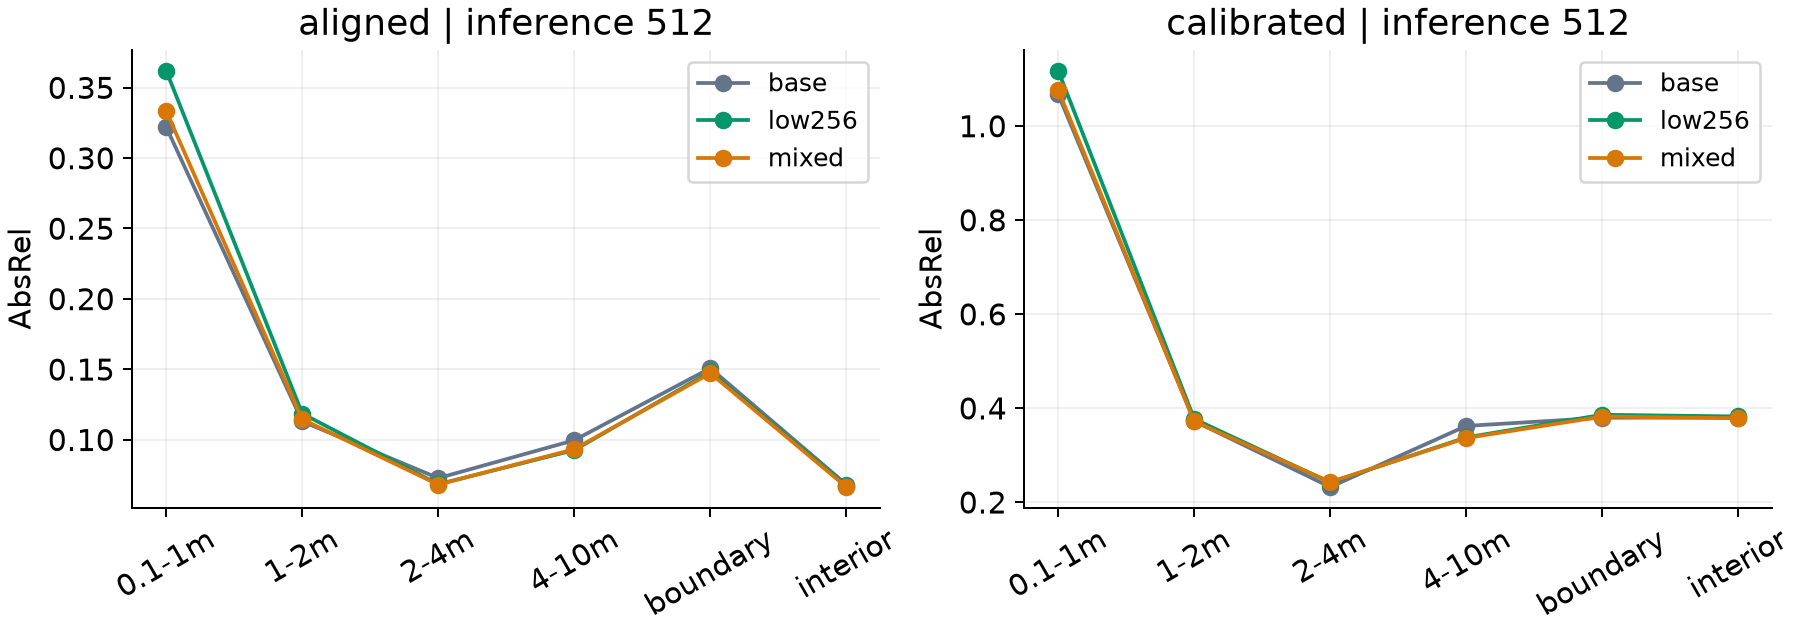
\includegraphics[width=\textwidth]{figures/failure_strata.png}
\caption{Exploratory external error strata at 512 inference. Left: per-image GT-aligned AbsRel. Right: fixed-validation-calibrated AbsRel. The threshold and weighting rules are fixed in the extension protocol. Different ranges may include different scene counts; these curves do not constitute extra confirmatory tests.}
\label{fig:strata}
\end{figure*}

We preserve the first three manifest samples as outcome-independent qualitative examples. Figure~\ref{fig:failures} instead shows the three largest regressions of scene-mean mixed512 against original512, selected explicitly after measuring error. The displayed adapter is fixed to draw1/seed17, whereas selection averages all 15 runs. This distinction prevents a few difficult images from being mistaken for a representative sample or a failure frequency estimate.
The selected cases show doorway-boundary errors (ID125), smoothed chair structure (ID196), and errors in a cluttered computer room with missing measured depth (ID58).

\begin{figure*}[t]
\centering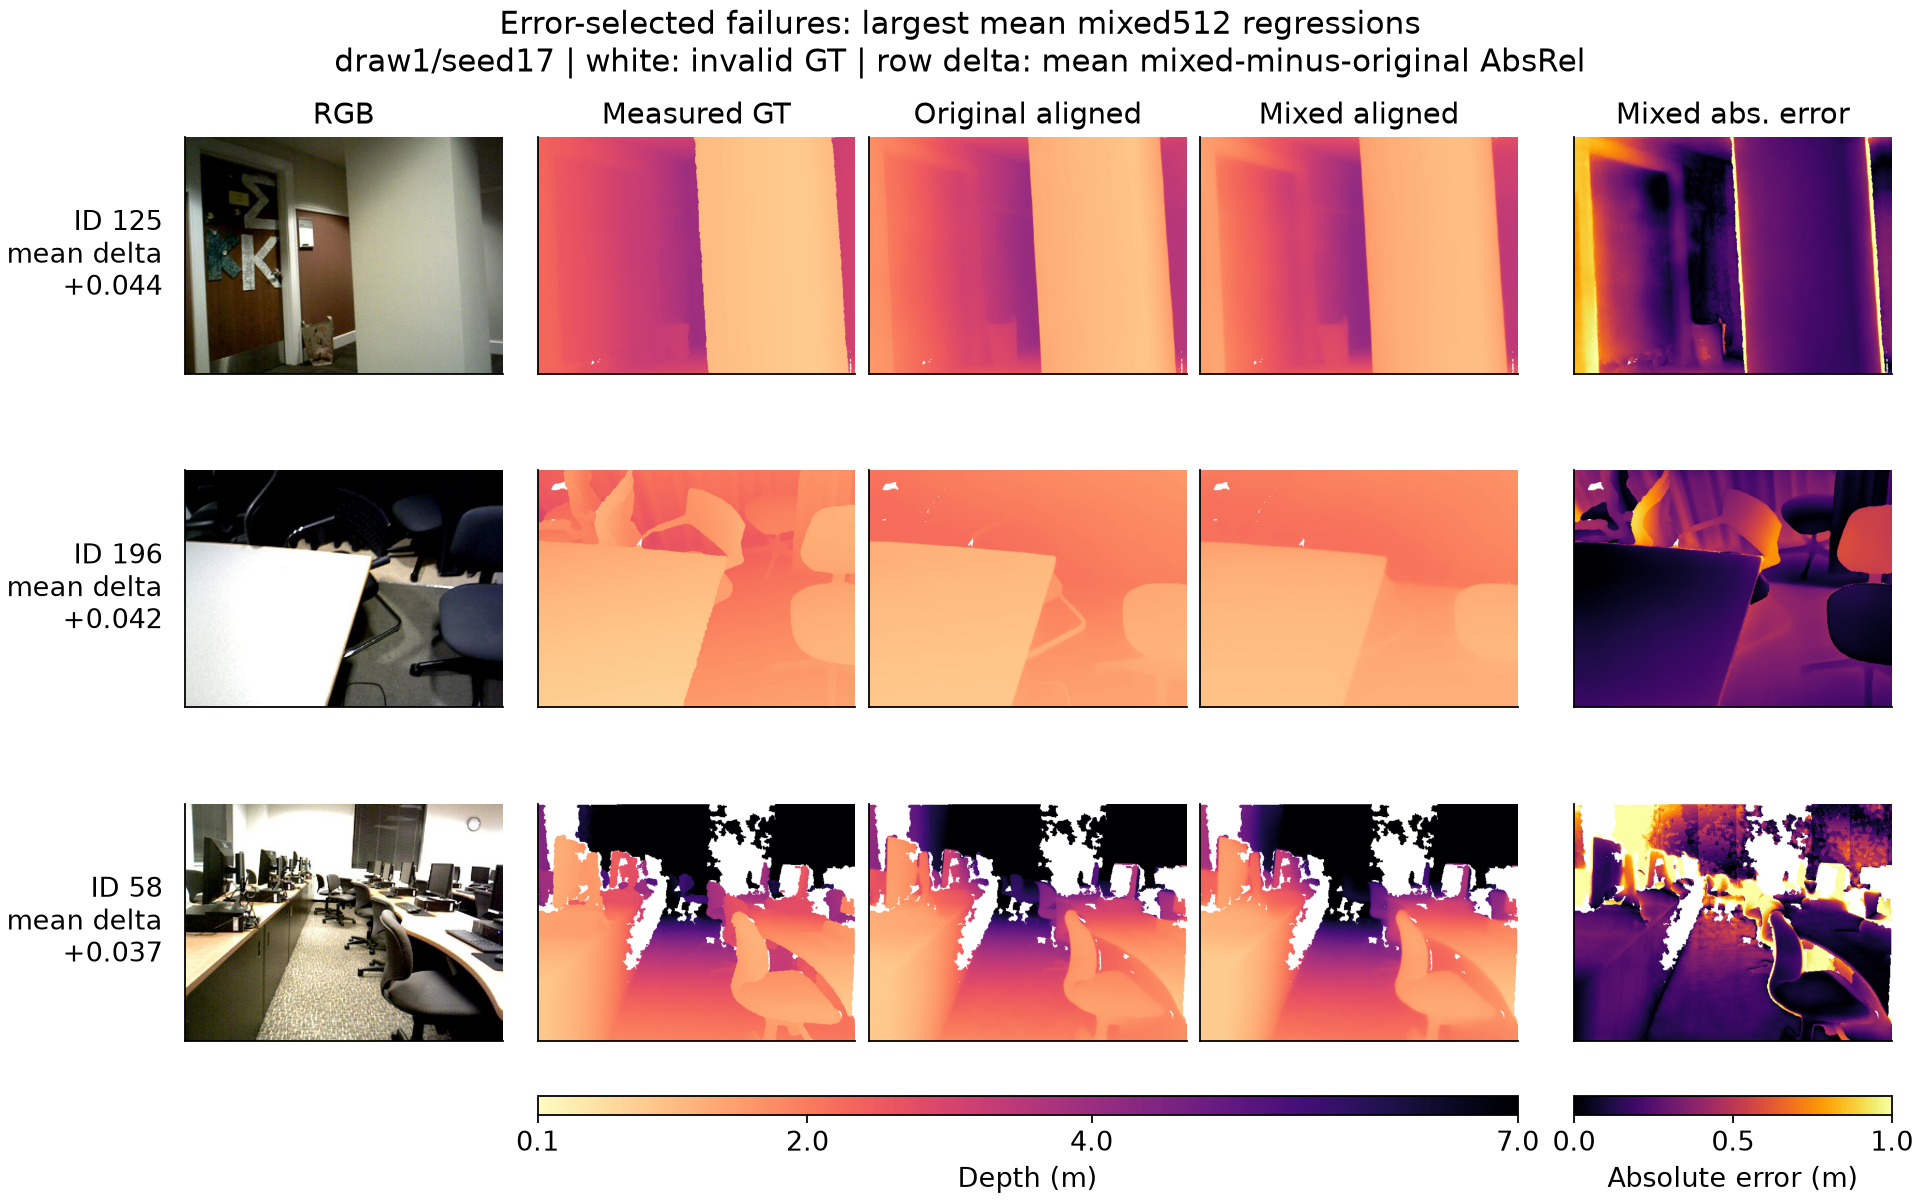
\includegraphics[width=.96\textwidth]{figures/selected_failures.png}
\caption{Explicitly error-selected failures. Rows are the three largest mean mixed512 regressions on the observed external cohort; the shown adapter is draw1/seed17. GT-aligned predictions use the target depth and therefore cannot demonstrate absolute-distance accuracy. Invalid measured pixels are masked.}
\label{fig:failures}
\end{figure*}

\subsection{Controlled cost and fixed-time validation}
The 30 replication trainings consumed 52.40 minutes of optimizer time, with peak allocated memory 2,512\,MiB. The frozen external predictions took 32.10 minutes of measured inference and peaked at 2,946.7\,MiB. These original timings exclude loading, caching and audits. The later low-only execution also contains isolated, extremely long wall-time readings. We retain those records but use the separate controlled benchmark for speed comparisons.

The separate benchmark measures original/mixed median latency of 66.71/73.41\,ms at 256 and 188.75/193.75\,ms at 512. All three adapter strategies are close: 73.41--73.59\,ms at 256 and 193.67--193.84\,ms at 512. Changing inference resolution has a much larger latency effect than choosing among these unmerged adapters. The 320 timed predictions exactly matched the stored outputs, verifying that warmup and measurement did not change the evaluated configuration. Within-run quantiles are descriptive and are not confidence intervals over hardware installations or independently selected checkpoints.

\begin{table}[t]
\centering\small
\caption{Fixed 120-second optimizer budget on draw1; validation32 only. Values are mean (sample SD) across three seeds. Update ranges show the achieved work within the budget.}
\label{tab:budget}
\begin{tabular}{lrrr}\toprule
Training & Updates & AbsRel@256 & AbsRel@512\\\midrule
Low-only & 405--454 & .0876 (.0025) & .0713 (.0015)\\
High-only & 405--422 & .1043 (.0029) & .0680 (.0009)\\
Mixed & 390--426 & .0904 (.0022) & .0696 (.0008)\\
\bottomrule\end{tabular}
\end{table}

Within the fixed-time diagnostic, low-only has the lowest mean error at 256 (0.08761 versus mixed 0.09041 and high-only 0.10431), while high-only has the lowest mean at 512 (0.06801 versus mixed 0.06963 and low-only 0.07132). Completed-update ranges overlap, so a fixed proportional speed advantage should not be assumed. These three-seed validation means again favor testing the deployment-matched schedule; they do not demonstrate general dominance. This comparison does not select a final checkpoint or reuse the external cohort as unseen confirmation. Equal optimizer-loop wall time also excludes different latent-cache costs and cannot be equated with equal total project time or equal energy.

\begin{figure*}[t]
\centering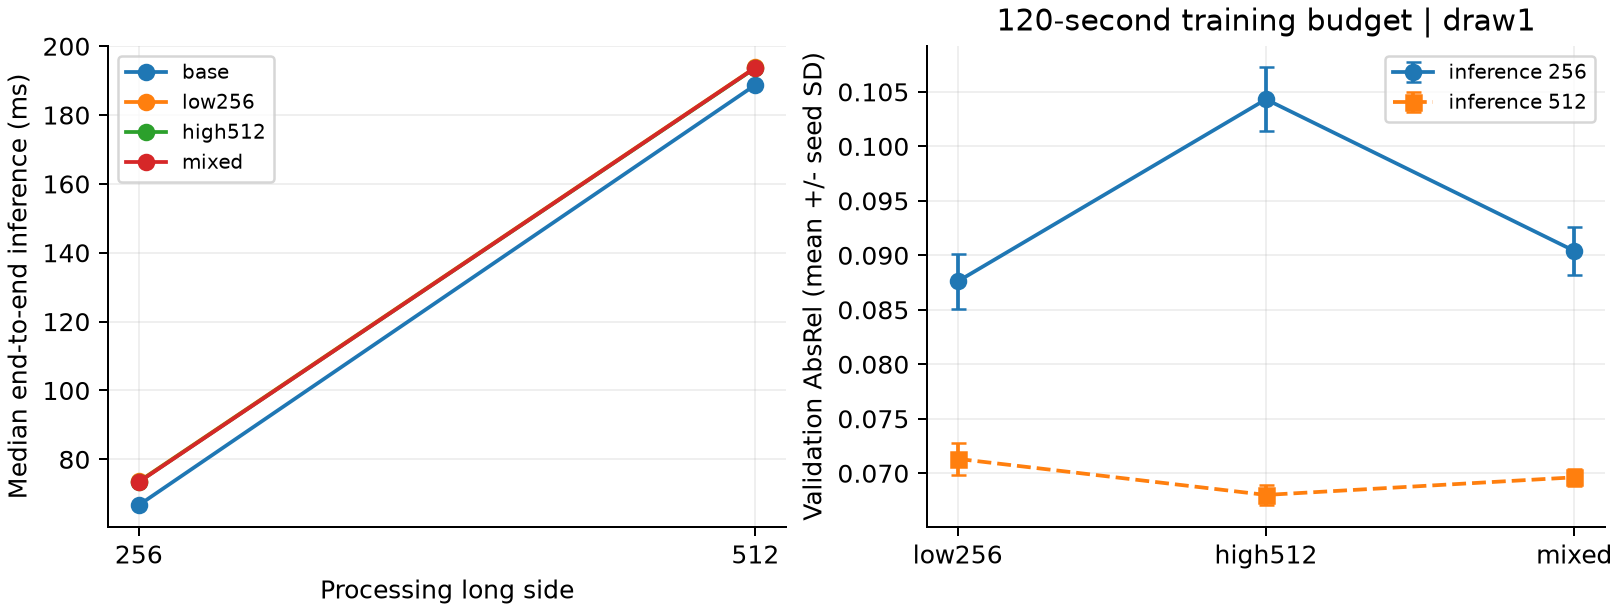
\includegraphics[width=\textwidth]{figures/controlled_cost.png}
\caption{Controlled local timing and the exploratory fixed-time training diagnostic. Left: inference medians across five randomized rounds and eight validation images. Right: validation AbsRel after 120 seconds of optimizer time, with SD across three seeds. Loading, caching and warmup are excluded; the timing scope is identical across conditions.}
\label{fig:cost}
\end{figure*}

\section{Discussion and Limitations}
The experiments show why a positive point estimate, a corrected statistical claim and a practical deployment advantage are different outcomes. Low-resolution relative-depth improvements are supported on the original frozen external cohort, while the 512 improvement is not. The added low-only control further constrains what can be attributed to mixing resolutions. Negative or inconclusive comparisons are informative because they rule out stronger interpretations of the project contribution.

The statistical evidence remains conditional on small numbers of training draws, overlapping training samples, selected indoor scenes and one inference noise seed per image. Location proxies are imperfect, and bootstrap p-values are approximate. The fixed calibration set is not resampled, so calibrated diagnostics do not include uncertainty from choosing a different calibration dataset. No result proves independence from all pretraining data or transfer to arbitrary cameras and outdoor scenes.

The method is deliberately modest: short LoRA training, cached latents, no image augmentation, one inference step and no new architecture. Our preservation term has a single tested weight; its weak result does not rule out all teacher regularizers. The specialist uses different supervision and input processing, and the compute-budget diagnostic covers only one training draw and a validation set. Remaining work could investigate metric-aware objectives, boundary-aware supervision or explicitly geometric consistency, with method selection confined to development data and a new frozen cohort for any confirmatory claim.

\section{Conclusion}
We built and audited a small-GPU depth-adaptation pipeline, progressing from exploratory ablations to replicated training and a fixed external evaluation. Mixed-resolution LoRA improves relative depth at 256 inference on the frozen external cohort, but its 512 advantage over original Marigold and accurate absolute-distance prediction are not established. The matched low-only control is stronger at 256 on the observed external cohort, and the fixed-time validation diagnostic favors different fixed schedules at the two inference resolutions. Mixing is therefore not a uniformly superior adaptation rule. The study identifies conditional accuracy, resolution, calibration and cost tradeoffs while retaining unsuccessful variants and the limits of the evidence.

\paragraph{Reproducibility.}
The separate supplement contains our source code, pinned dependency/model identifiers, protocols, small result summaries and execution instructions, excluding weights and raw datasets. Prediction metrics, input decoding, checkpoint restoration and historical-result preservation were audited. The code archive is below the course's 10\,MB limit. No previously frozen result file is overwritten by an exploratory extension.

{\small\begin{thebibliography}{12}
\bibitem{marigold} Bingxin Ke et al. Repurposing diffusion-based image generators for monocular depth estimation. In \emph{CVPR}, 2024.
\bibitem{marigold25} Bingxin Ke et al. Marigold: Affordable adaptation of diffusion-based image generators for image analysis. arXiv:2505.09358, 2025.
\bibitem{banana} Valentin Gabeur et al. Image generators are generalist vision learners. arXiv:2604.20329v1, 2026.
\bibitem{lora} Edward J. Hu et al. LoRA: Low-rank adaptation of large language models. In \emph{ICLR}, 2022.
\bibitem{resadapter} Jiaxiang Cheng et al. ResAdapter: Domain consistent resolution adapter for diffusion models. In \emph{AAAI}, 2025.
\bibitem{wise} Mitchell Wortsman et al. Robust fine-tuning of zero-shot models. In \emph{CVPR}, 2022.
\bibitem{dav2} Lihe Yang et al. Depth Anything V2. In \emph{NeurIPS}, 2024.
\bibitem{nyu} Nathan Silberman, Derek Hoiem, Pushmeet Kohli, and Rob Fergus. Indoor segmentation and support inference from RGBD images. In \emph{ECCV}, 2012.
\bibitem{sunrgbd} Shuran Song, Samuel P. Lichtenberg, and Jianxiong Xiao. SUN RGB-D: A RGB-D scene understanding benchmark suite. In \emph{CVPR}, 2015.
\bibitem{sun3d} Jianxiong Xiao, Andrew Owens, and Antonio Torralba. SUN3D: A database of big spaces reconstructed using SfM and object labels. In \emph{ICCV}, 2013.
\bibitem{holm} Sture Holm. A simple sequentially rejective multiple test procedure. \emph{Scandinavian Journal of Statistics}, 6(2):65--70, 1979.
\end{thebibliography}}
\end{document}
